
\documentclass[article,11pt]{article}

\usepackage{fullpage}
\usepackage{url}
\usepackage[english]{babel}
\usepackage[utf8]{inputenc}
\usepackage{amsmath}
\usepackage{bm, amssymb}
\usepackage{graphicx}
\graphicspath{ {/} }\\
\usepackage{listings}
\setlength\parindent{24pt}

\title{ELEC-E7851 - Computational User Interface Design \\ Task 3.2}
\begin{document}
\date{}
\maketitle

According to the article, the variables $ \beta $ and $ F_{cmin} $ should be adjusted accordingly: $ \beta $ for reducing lag and $ F_{cmin} $ for reducing jittering.\newline

The values were found in the noise.py in the following block (below example with the values I chose) and were clearly marked with the FIXME. A third FIXME was found earlier in the code, but that one seemed to be okay if left untouched.\newline

The values I picked were chosen by plotting the filtered signal against the raw signal and comparing when the jittering and lag seemed to be within appropriate limits. First, $ F_{cmin} $ was adjusted to its value and then $ \beta $ was adjusted to reduce the lag caused by $ F_{cmin} $. Some lag and jittering still exist, but I felt that they were both within acceptable limits.

\begin{lstlisting}
    config = {
        'freq': 650,       # Hz
        'mincutoff': 0.007,  # FIXME
        'beta': 0.005,       # FIXME
        'dcutoff': 1.0     # this one should be ok
        }
\end{lstlisting}

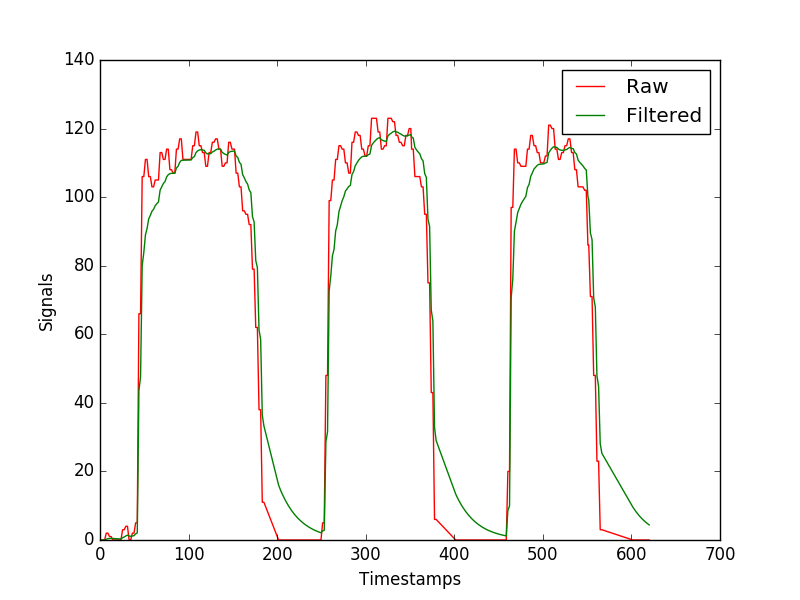
\includegraphics[scale=0.5]{figure_1}

\end{document}